% Options for packages loaded elsewhere
\PassOptionsToPackage{unicode}{hyperref}
\PassOptionsToPackage{hyphens}{url}
%
\documentclass[
]{article}
\usepackage{amsmath,amssymb}
\usepackage{lmodern}
\usepackage{iftex}
\ifPDFTeX
  \usepackage[T1]{fontenc}
  \usepackage[utf8]{inputenc}
  \usepackage{textcomp} % provide euro and other symbols
\else % if luatex or xetex
  \usepackage{unicode-math}
  \defaultfontfeatures{Scale=MatchLowercase}
  \defaultfontfeatures[\rmfamily]{Ligatures=TeX,Scale=1}
\fi
% Use upquote if available, for straight quotes in verbatim environments
\IfFileExists{upquote.sty}{\usepackage{upquote}}{}
\IfFileExists{microtype.sty}{% use microtype if available
  \usepackage[]{microtype}
  \UseMicrotypeSet[protrusion]{basicmath} % disable protrusion for tt fonts
}{}
\makeatletter
\@ifundefined{KOMAClassName}{% if non-KOMA class
  \IfFileExists{parskip.sty}{%
    \usepackage{parskip}
  }{% else
    \setlength{\parindent}{0pt}
    \setlength{\parskip}{6pt plus 2pt minus 1pt}}
}{% if KOMA class
  \KOMAoptions{parskip=half}}
\makeatother
\usepackage{xcolor}
\IfFileExists{xurl.sty}{\usepackage{xurl}}{} % add URL line breaks if available
\IfFileExists{bookmark.sty}{\usepackage{bookmark}}{\usepackage{hyperref}}
\hypersetup{
  pdftitle={Assignment 2: Interpreting Quantitative Findings},
  hidelinks,
  pdfcreator={LaTeX via pandoc}}
\urlstyle{same} % disable monospaced font for URLs
\usepackage[margin=1in]{geometry}
\usepackage{graphicx}
\makeatletter
\def\maxwidth{\ifdim\Gin@nat@width>\linewidth\linewidth\else\Gin@nat@width\fi}
\def\maxheight{\ifdim\Gin@nat@height>\textheight\textheight\else\Gin@nat@height\fi}
\makeatother
% Scale images if necessary, so that they will not overflow the page
% margins by default, and it is still possible to overwrite the defaults
% using explicit options in \includegraphics[width, height, ...]{}
\setkeys{Gin}{width=\maxwidth,height=\maxheight,keepaspectratio}
% Set default figure placement to htbp
\makeatletter
\def\fps@figure{htbp}
\makeatother
\setlength{\emergencystretch}{3em} % prevent overfull lines
\providecommand{\tightlist}{%
  \setlength{\itemsep}{0pt}\setlength{\parskip}{0pt}}
\setcounter{secnumdepth}{5}
\newlength{\cslhangindent}
\setlength{\cslhangindent}{1.5em}
\newlength{\csllabelwidth}
\setlength{\csllabelwidth}{3em}
\newlength{\cslentryspacingunit} % times entry-spacing
\setlength{\cslentryspacingunit}{\parskip}
\newenvironment{CSLReferences}[2] % #1 hanging-ident, #2 entry spacing
 {% don't indent paragraphs
  \setlength{\parindent}{0pt}
  % turn on hanging indent if param 1 is 1
  \ifodd #1
  \let\oldpar\par
  \def\par{\hangindent=\cslhangindent\oldpar}
  \fi
  % set entry spacing
  \setlength{\parskip}{#2\cslentryspacingunit}
 }%
 {}
\usepackage{calc}
\newcommand{\CSLBlock}[1]{#1\hfill\break}
\newcommand{\CSLLeftMargin}[1]{\parbox[t]{\csllabelwidth}{#1}}
\newcommand{\CSLRightInline}[1]{\parbox[t]{\linewidth - \csllabelwidth}{#1}\break}
\newcommand{\CSLIndent}[1]{\hspace{\cslhangindent}#1}
\usepackage{amsmath}
\usepackage{booktabs}
\usepackage{floatrow}
\floatsetup[figure]{capposition=top}
\floatsetup[table]{capposition=top}
\usepackage{booktabs}
\usepackage{longtable}
\usepackage{array}
\usepackage{multirow}
\usepackage{wrapfig}
\usepackage{float}
\usepackage{colortbl}
\usepackage{pdflscape}
\usepackage{tabu}
\usepackage{threeparttable}
\usepackage{threeparttablex}
\usepackage[normalem]{ulem}
\usepackage{makecell}
\usepackage{xcolor}
\ifLuaTeX
  \usepackage{selnolig}  % disable illegal ligatures
\fi

\title{Assignment 2: Interpreting Quantitative Findings}
\usepackage{etoolbox}
\makeatletter
\providecommand{\subtitle}[1]{% add subtitle to \maketitle
  \apptocmd{\@title}{\par {\large #1 \par}}{}{}
}
\makeatother
\subtitle{\hfill\break
University of Glasgow\\
\strut \\
Student ID: 2819052\\
Course: Quantitative Methods\\
Number of words: 381}
\author{}
\date{\vspace{-2.5em}}

\begin{document}
\maketitle

\pagebreak

\setcounter{tocdepth}{2}
\tableofcontents

\pagebreak

\hypertarget{introduction}{%
\section{Introduction}\label{introduction}}

In 1998, the Good Friday/Belfast Agreement was signed and later
validated by the voters, and this agreement marked a new era of hope
towards peace, equality, and inclusion in Northern Ireland
(\protect\hyperlink{ref-galligan2013gender}{Galligan 2013}). The main
focus on the agreement and referendum was obviously to stop the violent
conflict and seek peace, but one part of the agreement also emphasized
an equality agenda (\protect\hyperlink{ref-Hayward2021}{Hayward 2021}).
Thus, the agreement also marked the first Northern Irish formal
recognition of women's rights to political inclusion
(\protect\hyperlink{ref-galligan2013gender}{Galligan 2013}). However, a
formal recognition does not necessarily imply that gender equality
trickles down into social norms and practices. Therefore, this report
examines the contemporary state of women's equality in Northern Ireland.

Perhaps, the most central concept within gender equality is the
\emph{gender pay gap}. Disparities in income is an important indicator
for gender equality, because it has social, economic, and physiological
consequences (\protect\hyperlink{ref-bishu2017gender}{Bishu and Alkadry
2017}). Research on this area have identified several factors that seems
to influence a gender pay gap. One such factor can be inequality in
access to workplace authority, where women are denied manager or
supervisor position although there were equally qualified
(\protect\hyperlink{ref-bishu2017gender}{Bishu and Alkadry 2017}). Other
factors can be discrimination in hiring or promotion processes, but also
lack of gender representation can avoid minorities to even apply for a
job or promition (\protect\hyperlink{ref-bishu2017gender}{Bishu and
Alkadry 2017}).

Deductive (\protect\hyperlink{ref-bryman2016social}{Bryman 2016, 33})

\hypertarget{data-and-method}{%
\section{Data and method}\label{data-and-method}}

We employ a cross-sectional design
(\protect\hyperlink{ref-bryman2016social}{Bryman 2016, 53})

\hypertarget{sample-and-data-collection}{%
\subsection{Sample and Data
Collection}\label{sample-and-data-collection}}

Two-tailed t-test {[}fogarty2018quantitative 156{]} Chi-squared test
{[}fogarty2018quantitative 176{]} Multiple linear regression with OLS
{[}fogarty2018quantitative 192ff{]}

\begin{table}[H]

\caption{\label{tab:unnamed-chunk-1}Descriptive Statistics for Cleaned and Full Sample (Categorical Variables)}
\centering
\begin{tabular}[t]{llllll}
\toprule
\multicolumn{1}{c}{ } & \multicolumn{2}{c}{Cleaned Sample} & \multicolumn{2}{c}{Full Sample} & \multicolumn{1}{c}{ } \\
\cmidrule(l{3pt}r{3pt}){2-3} \cmidrule(l{3pt}r{3pt}){4-5}
Variable & N & Percent & N & Percent & Test\\
\midrule
Sex & 675 &  & 1204 &  & X2=1.022\\
... Male & 284 & 42.1\% & 537 & 44.6\% & \\
... Female & 391 & 57.9\% & 667 & 55.4\% & \\
Religion & 675 &  & 1168 &  & X2=0.849\\
... Catholic & 277 & 41\% & 491 & 42\% & \\
\addlinespace
... Protestant & 283 & 41.9\% & 497 & 42.6\% & \\
... No religion & 115 & 17\% & 180 & 15.4\% & \\
Sexual Orientation & 675 &  & 1191 &  & X2=3.039\\
... I am heterosexual or straight & 657 & 97.3\% & 1173 & 98.5\% & \\
... I am gay or lesbian (homosexual) & 14 & 2.1\% & 14 & 1.2\% & \\
\addlinespace
... I am bi-sexual & 2 & 0.3\% & 2 & 0.2\% & \\
... Other & 2 & 0.3\% & 2 & 0.2\% & \\
Constitutional View & 675 &  & 1183 &  & X2=0.347\\
... Unionist & 199 & 29.5\% & 348 & 29.4\% & \\
... Nationalist & 138 & 20.4\% & 255 & 21.6\% & \\
\addlinespace
... Neither & 338 & 50.1\% & 580 & 49\% & \\
Trade union membership & 675 &  & 1179 &  & X2=9.162***\\
... Yes & 301 & 44.6\% & 440 & 37.3\% & \\
... No & 374 & 55.4\% & 739 & 62.7\% & \\
Supervisor: No & 675 &  & 883 &  & X2=0.143\\
\addlinespace
... Yes & 211 & 31.3\% & 267 & 30.2\% & \\
... No & 464 & 68.7\% & 616 & 69.8\% & \\
\bottomrule
\multicolumn{6}{l}{\rule{0pt}{1em}\textit{Note: }}\\
\multicolumn{6}{l}{\rule{0pt}{1em}Statistical significance markers: * p<0.1; ** p<0.05; *** p<0.01}\\
\end{tabular}
\end{table}

\begin{table}[H]

\caption{\label{tab:unnamed-chunk-1}Descriptive Statistics for Cleaned and Full Sample (Numerical Variables)}
\centering
\begin{tabular}[t]{llllllll}
\toprule
\multicolumn{1}{c}{ } & \multicolumn{3}{c}{Cleaned Sample} & \multicolumn{3}{c}{Full Sample} & \multicolumn{1}{c}{ } \\
\cmidrule(l{3pt}r{3pt}){2-4} \cmidrule(l{3pt}r{3pt}){5-7}
Variable & N & Mean & SD & N & Mean & SD & Test\\
\midrule
Annual Personal Income (GBP) & 675 & 16892.089 & 13447.704 & 897 & 16394.582 & 13465.9 & F=0.526\\
Age & 675 & 46.763 & 17.117 & 1201 & 49.615 & 18.53 & F=10.81***\\
\bottomrule
\multicolumn{8}{l}{\rule{0pt}{1em}\textit{Note: }}\\
\multicolumn{8}{l}{\rule{0pt}{1em}Statistical significance markers: * p<0.1; ** p<0.05; *** p<0.01}\\
\end{tabular}
\end{table}

\hypertarget{dependent-and-independent-variables}{%
\subsection{Dependent and Independent
Variables}\label{dependent-and-independent-variables}}

Levels of measurement: nominal, ordinal, interval, and ratio
(\protect\hyperlink{ref-fogarty2018quantitative}{Fogarty 2018, 56})

\begin{figure}[H]

{\centering 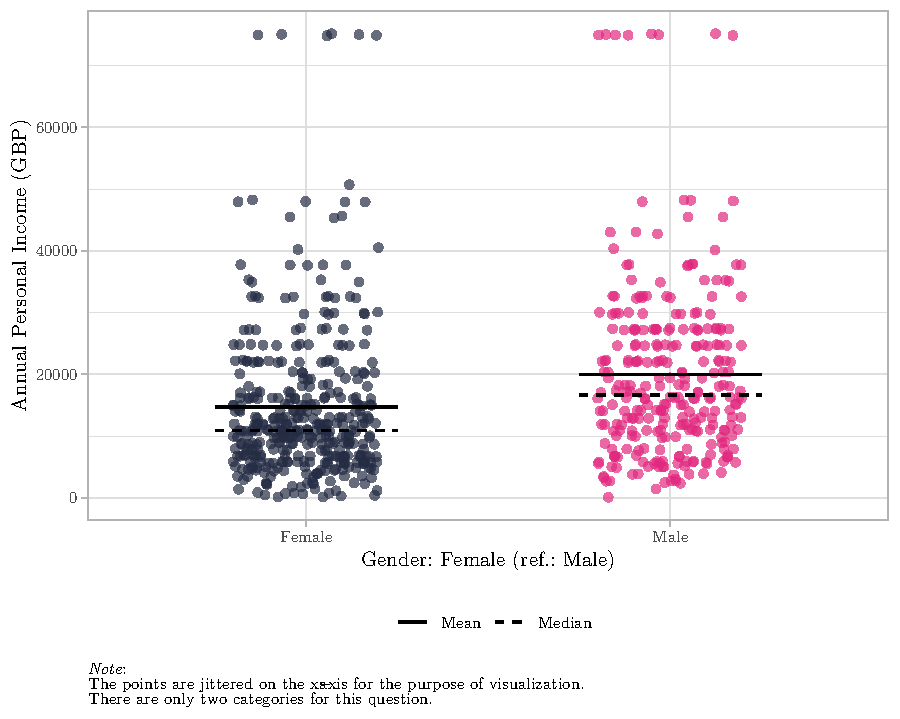
\includegraphics[width=0.8\linewidth]{paper_files/figure-latex/unnamed-chunk-2-1} 

}

\caption{Scatterplot of Income and Sex}\label{fig:unnamed-chunk-2}
\end{figure}

\hypertarget{results-and-discussion}{%
\section{Results and discussion}\label{results-and-discussion}}

Here comes the regression.

\begin{table}[H] \centering 
  \caption{Regression results} 
  \label{} 
\small 
\begin{tabular}{@{\hspace{5pt}}l@{\hspace{5pt}}c} 
\toprule 
 & \multicolumn{1}{c}{Dependent Variable} \\ 
\cmidrule(rr){2-2} 
 & Annual Personal Income (GBP) \\ 
\midrule  
\\[-2.1ex] Sex: Female (ref.: Male) & $-$5,068.737$^{***}$ \\ 
  & (994.748) \\ 
 \addlinespace 
 Religion: Protestant (ref.: Catholic) & 465.188 \\ 
  & (1,458.367) \\ 
 \addlinespace 
 Religion: No religion & 895.169 \\ 
  & (1,533.323) \\ 
 \addlinespace 
 Sexual Orientation: Homosexual (ref.: Heterosexual) & $-$6,247.777$^{*}$ \\ 
  & (3,437.048) \\ 
 \addlinespace 
 Sexual Orientation: bi-sexual & $-$2,826.980 \\ 
  & (8,698.806) \\ 
 \addlinespace 
 Sexual Orientation: Other & 1,323.336 \\ 
  & (8,737.282) \\ 
 \addlinespace 
 Constitutional View: Nationalist (ref.: Unionist) & 1,788.873 \\ 
  & (1,898.294) \\ 
 \addlinespace 
 Constitutional view: Neither & 1,438.036 \\ 
  & (1,350.423) \\ 
 \addlinespace 
 Trade union membership: No (ref.: Yes) & $-$5,277.978$^{***}$ \\ 
  & (977.008) \\ 
 \addlinespace 
 Supervisor: No (ref.: Yes) & $-$8,648.320$^{***}$ \\ 
  & (1,037.559) \\ 
 \addlinespace 
 Age & $-$84.369$^{***}$ \\ 
  & (29.430) \\ 
 \addlinespace 
 Constant & 31,343.540$^{***}$ \\ 
  & (2,488.067) \\ 
 \addlinespace 
\midrule  
Observations & 675 \\ 
R$^{2}$ & 0.183 \\ 
Adjusted R$^{2}$ & 0.170 \\ 
Residual Std. Error & 12,252.840 (df = 663) \\ 
F Statistic & 13.533$^{***}$ (df = 11; 663) \\ 
\bottomrule 
\textit{Note:}  & \multicolumn{1}{r}{$^{*}$p$<$0.1; $^{**}$p$<$0.05; $^{***}$p$<$0.01} \\ 
\end{tabular} 
\end{table}

Influential data points / outliers {[}fogarty2018quantitative 221-222{]}

\hypertarget{check-for-heteroscedasticity}{%
\subsection{Check for
Heteroscedasticity}\label{check-for-heteroscedasticity}}

Here comes a check for heteroscedasticity.

\begin{figure}[H]

{\centering 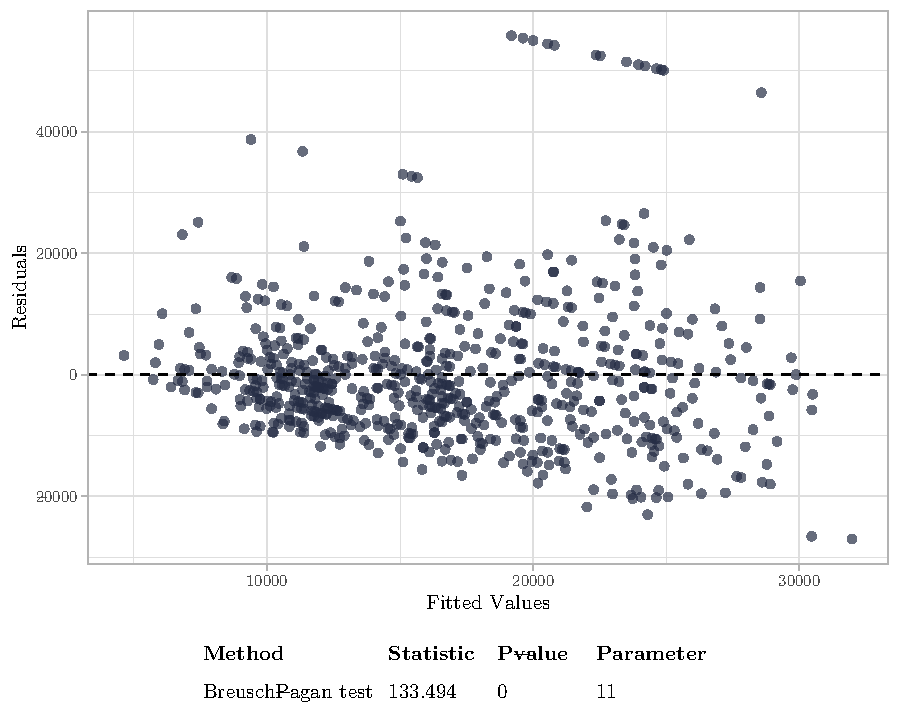
\includegraphics[width=0.8\linewidth]{paper_files/figure-latex/unnamed-chunk-4-1} 

}

\caption{Scatterplot of Fitted Values and Residuals}\label{fig:unnamed-chunk-4}
\end{figure}

\hypertarget{reliability-and-validity}{%
\subsection{Reliability and Validity}\label{reliability-and-validity}}

Reliability and validity
(\protect\hyperlink{ref-bryman2016social}{Bryman 2016, 41}) Internal and
external validity (\protect\hyperlink{ref-bryman2016social}{Bryman 2016,
41--42})

\hypertarget{conclusion}{%
\section{Conclusion}\label{conclusion}}

\pagebreak

\hypertarget{references}{%
\section*{References}\label{references}}
\addcontentsline{toc}{section}{References}

\hypertarget{refs}{}
\begin{CSLReferences}{1}{0}
\leavevmode\vadjust pre{\hypertarget{ref-bishu2017gender}{}}%
Bishu, Sebawit G., and Mohamad G. Alkadry. 2017. {``A Systematic Review
of the Gender Pay Gap and Factors That Predict It.''}
\emph{Administration \& Society} 49 (1): 65--104.
\url{https://doi.org/10.1177/0095399716636928}.

\leavevmode\vadjust pre{\hypertarget{ref-bryman2016social}{}}%
Bryman, A. 2016. \emph{Social Research Methods}. Oxford University
Press. \url{https://books.google.co.uk/books?id=N2zQCgAAQBAJ}.

\leavevmode\vadjust pre{\hypertarget{ref-fogarty2018quantitative}{}}%
Fogarty, B. J. 2018. \emph{Quantitative Social Science Data with r: An
Introduction}. Core Textbook. SAGE Publications.
\url{https://books.google.co.uk/books?id=jwJ6DwAAQBAJ}.

\leavevmode\vadjust pre{\hypertarget{ref-galligan2013gender}{}}%
Galligan, Yvonne. 2013. {``Gender and Politics in Northern Ireland: The
Representation Gap Revisited.''} \emph{Irish Political Studies} 28 (3):
413--33.

\leavevmode\vadjust pre{\hypertarget{ref-Hayward2021}{}}%
Hayward, Katy. 2021. {``The 1998 Good Friday (Belfast) Agreement
Referendums in Northern Ireland and the Republic of Ireland.''} In
\emph{The Palgrave Handbook of European Referendums}, edited by Julie
Smith, 247--65. Cham: Springer International Publishing.
\url{https://doi.org/10.1007/978-3-030-55803-1_12}.

\end{CSLReferences}

\end{document}
